%%% Thesis Introduction --------------------------------------------------
\chapter{From Stochastic Equations to Deterministic Average Equations}
\ifpdf
    \graphicspath{{FromStochastic/Figs/PNG/}{FromStochastic/Figs/PDF/}{Fromstochastic/Figs/}}
\else
    \graphicspath{{FromStochastic/Figs/EPS/}{FromStochastic/Figs/}}
\fi
In the literature we find differential equations for growth  processes, such as: protein production and degradation, predator-prey dynamics such as the Lolka-Volterra equations and selection dynamics as Eq. \eqref{3.12}. These are deterministic descriptions of those processes, which really are stochastic. What these equations are telling us is about the average behavior of those systems, but how can those equations be derived from the master equation Eq. \eqref{4.1}? Many of these differential equations have been proposed without a direct explanation of their relation with the implicit stochastic process \cite{Traulsen2005a}. For example, the equation 
\begin{equation}\label{6.1}
\frac{dx_i}{dt}=x_i(\pi_i(x) - \bar\pi)
\end{equation}  
for replication dynamics in evolutionary game theory is not the result from averaging over the master equation of its respective Moran process. This also happens with random drift and Eq. \eqref{3.12}, where the average of the stochastic simulation does not fit with the solution of this equation.  

In this section  a simple approach to derive the average differential of some simple stochastic systems will be shown, such as that of protein creation and degradation and for more difficult master equation as those that result in Moran process for evolutionary dynamics, using Focker-Planck approximation and Langevin equation.
\section{A Simple Example: Protein creation and degradation}
Inside any cell there is a genetic system that is  responsible for the production of the proteins that the cell needs. Suppose that the expression rate of protein is $\gamma$, but inside of cell this proteins also have a degradation, that can be represented by the rate $\beta$. Because of the stochasticity these rates represents the probabilities by unit time of creation or degradation.
Taking $1$ as the time step and assuming it is small enough compared to $\gamma$ and $\beta$ that just one events happens at each time step\cite{Pedraza1,Thattai},  the master equation  for the state of $i$ proteins is
\begin{equation}\label{6.2}
\frac{dp_i(t)}{dt}=-(\gamma + i\beta)p_i(t) + (i+1)\beta p_{i+1}(t) + \gamma p_{i-1}(t).
\end{equation} 
where $i$ goes from $0$ to $\infty$ and the average of $i$ is represented by
\begin{equation}
\langle i\rangle=\sum\limits_{i=0}^{i=\infty}ip_i (t).
\end{equation}
Averaging over Eq. \eqref{6.2} we get
\begin{equation}
\frac{d \langle i\rangle}{dt}=-\sum\limits_{i=0}^{i=\infty}i(\gamma + i\beta)p_i(t) + \sum\limits_{i=0}^{i=\infty}i(i+1)\beta p_{i+1}(t) + \sum\limits_{i=0}^{i=\infty}i \gamma p_{i-1}(t).
\end{equation}
and replacing the next summations in the above equation
\begin{equation}
\sum\limits_{i=0}^{\infty}i\gamma p_{i-1}(t)=\sum\limits_{i=0}^{\infty}(i+1)\gamma p_{i}(t)\;\;\; 	\sum\limits_{i=0}^{\infty}i(i+1)\beta p_{i+1}(t)
\end{equation} 
the average  simplifies to the differential equation
\begin{equation}
\frac{d \langle i\rangle}{dt} = \gamma - \beta \langle i \rangle.
\end{equation}
Which has the solution
\begin{equation}
\langle i \rangle =\frac{\gamma}{\beta}+\left(\langle i\rangle_0 -\frac{\gamma}{\beta}\right)e^{-\beta t}
\end{equation}
and the average protein number $\langle i\rangle=\gamma/\beta$ in steady state.

We can also determine the steady state protein distribution by taking $\frac{dp_i(t)}{dt}=0$ in the master equation
\begin{equation}
0=-(\gamma + i\beta)p_i(t) + (i+1)\beta p_{i+1}(t) + \gamma p_{i-1}(t),
\end{equation}
which can be written as
\begin{equation}
(i+1)p_{i+1}-\langle i\rangle p_i = i p_i - \langle i \rangle p_{i-1}.
\end{equation} 
 Setting $y_i=i p_i - \langle i \rangle p_{i-1}$ and using the above equation, the sum over $y_i$ is
\begin{equation}
\sum\limits_{i=0}^{\infty}y_i =0.
\end{equation} 
Then $y_i$ must be $0$, and the recurrence equation for $p_i$ is
\begin{equation}
p_i = \frac{\langle i \rangle}{i} p_{i-1}
\end{equation}
Therefore
\begin{equation}
p_i=\frac{\langle i\rangle^i}{i!}p_0.
\end{equation}
Because of $\sum\limits_{i=0}^{\infty}p_i=1$ and $\sum\langle i \rangle^i / i!=e^{\langle i \rangle}$, $p_0=e^{\langle i \rangle}$ and finally
\begin{equation}
p_i =\frac{\langle i \rangle ^i}{i!}e^{-\langle i\rangle}.
\end{equation}
 The steady state of proteins have a Poisson distribution, which for large $\langle i \rangle$ can be approximated to a continuos Gaussian distribution.
   
These two results; the deterministic law and steady state distribution, were simple to determinate due to the lineal form of the transition rates $P_{i,i+1}$ and $P_{i,i-1}$ of this system; but even then, the dynamical distribution is difficult to calculate analytically. Next we will see some approximation methods to calculate the deterministic law when the transition probabilities are not lineal.  
\section{Average Differential Equations in Evolutionary Dynamics}
In this section  an approximation method to find deterministic differential equations from stochastic systems, where the transition probabilities are non-linear functions of the stochastic state variable $i$, will be explained.  

In evolutionary dynamics we have transition probabilities that are not linear function of the population frequency $i$, which have the form
\begin{equation}
P_{i,i+1}=\frac{1-w+w\pi_C}{1-w+w\langle \pi \rangle}\frac{i}{n}\frac{n-i}{n}\;\;\; P_{i,i-1}=\frac{1-w+w\pi_D}{1-w+w\langle \pi \rangle}\frac{i}{n}\frac{n-i}{n}.
\end{equation}
Introducing these transitions into the  master equation  
\begin{equation}
\frac{d P_{i}(t)}{dt}=-(P_{i,i+1} + P_{i.i-1})P_{i}(t) + P_{i+1,i}P_{i+1}(t)+ P_{i-1,i}P_{i-1}(t),
\end{equation}
and averaging over all the systems we will find terms of the form
\begin{equation}
\sum\limits_{i=0}^{n}\frac{1-w+w\pi(i)_C}{1-w+w\langle \pi(i) \rangle}\frac{i}{n}\frac{n-i}{n} i P_{i}(t),
\end{equation}
which need to be transformed to get averages of $i$, and write the average differential equation as
\begin{equation}
\frac{d\langle i \rangle}{dt}=f(\langle i \rangle,\langle i \rangle^2, .., \langle i \rangle^m).
\end{equation}  
This method to obtain the deterministic law is difficult. However it is possible to use a easier method using the relation between Fokker-Planck equation and Langevin equation.

 
First, to determine the Fokker -Planck equation, let us set $P_{i,i+1}=P_{i}^{+}$ and $P_{i,i-1}=P_{i}^{-}$, and consider the case where $i$ is large and behaves as a continuos variable. We can then write the transition probabilities as
\begin{equation}
P_{i}^{+}=P^{+}(i)\;\;\; and \;\;\; P_{i}^{-}=P^{-}(i).
\end{equation}  
Expanding the terms $P(i\pm 1,t)$, $P^{+}(i\pm1)$ and $P^{-}(i\pm1)$ as a Taylor series up to second order, the Fokker-Planck equation for the Moran process(one step process) is\cite{Traulsen2005a}
\begin{equation}\label{6.19}
\frac{\partial P(i,t)}{\partial t}=-\frac{\partial}{\partial i}\left[\left(P^{+}(i)-P^{-}(i)\right)P(i,t)-\frac{1}{2}\frac{\partial}{\partial i}\left(P^{+}(i)+P^{-}(i)\right)P(i,t)\right].
\end{equation} 
This equation is often used to calculate the probability distribution and averages in steady state. This can also be done with the Langevin approach.

Langevin proposed an stochastic differential equation of the form
\begin{equation}\label{6.20}
\frac{di}{dt}=a(i,t) + b(i,t)\xi(t),
\end{equation}
that have a deterministic part $a(i,t)$ and the stochastic $b(i,t)\xi(t)$, where $\xi(t)$ is an uncorrelated time random variable with white noise $\langle\xi\rangle=0$. Since this is a Langevin approach for the Moran process, the quantities $a(i,t)$ and $b(i,t)$ must  satisfy the absorbing states $0$ and $n$, where $di/dt=0$. Therefore $a(i,t)=0$ and $b(i,t)=0$ for $i=0,n$. This tells us that these factors have a relation with the transition probabilities.

Ito's calculus lets us establish the equivalence between Langevin and Fokker-Plank\cite{Kampen, Gardiner}. For an  arbitrary function $f[i(t)]$,  Ito's formula for the expansion of the differential $df[i(t)]=f[i(t)+di(t)]-f[i(t)]$ is
\begin{equation}
df[i(t)]=\{a(i,t)\partial_{i}f+\frac{1}{2}b^2(i,t)\partial_{i}^{2}f\}dt+b(i,t)\partial_{i}f\xi dt.
\end{equation}  
Averaging this equation
\begin{equation}
\frac{d}{dt}\langle f[i(t)]\rangle=\langle a(i,t)\partial_{i}f+\frac{1}{2}b^2(i,t)\partial_{i}^{2}f\rangle + \langle b(i,t)\partial_{i}f\xi\rangle,
\end{equation}
where because of the irregularity of $\xi$, $\langle b(i,t)\partial_{i}f\xi\rangle=0$. Thus
\begin{equation}
\int f(i) \partial_{t}P(i,t) di=\int a(i,t)\partial_{i}f P(i,t) di +\int\frac{1}{2}b^2(i,t)\partial^{2}_{i}f P(i,t)di .
\end{equation}
 Integrating by parts this becomes
 \begin{equation}
 \int f \partial_{t}Pdi=aPf\mid-\int\partial_{i}(aP)fdi + \frac{1}{2}b^{2}P\partial_{i}f\mid -\int\frac{1}{2}\partial_{i}(b^2P)\partial_{i}f di 
 \end{equation} 
 and once again for the integral that contains $\partial_{i}f$
 \begin{equation}
  \int f \partial_{t}Pdi=aPf\mid-\int\partial_{i}(aP)fdi + \frac{1}{2}b^{2}P\partial_{i}f\mid - \frac{1}{2}\partial_{i}(b^2P)f\mid + \int\frac{1}{2}\partial^{2}_{i}(b^2P)fdi,
 \end{equation}  
  where the boundary terms banish because they  are evaluated in the absorbing states $i=0,n$. Therefore we obtain
  \begin{equation}
  \int \partial_{t}P f di=\int\left( -\partial_{i}(aP)+\frac{1}{2}\partial^{2}_{i}(b^2P)\right)fdi.
  \end{equation} 
 Since $f(i)$ is arbitrary, the integral terms correspond to Fokker-Planck equation
 \begin{equation}\label{6.27}
 \partial_{t}P(i,t)= -\partial_{i}(a(i,t)P(i,t))+\frac{1}{2}\partial^{2}_{i}(b^2(i,t)P(i,t)).
 \end{equation}  
 Notice that $f(i)$ can be $i(t)$. Then the Langevin equation
 \begin{equation}
 \frac{di}{dt}=a(i,t) + b(i,t)\xi(t)
 \end{equation} 
 is equivalent to Fokker-Planck Eq. \eqref{6.27}. Therfore by similitude  with Eq. \eqref{6.19}, the coefficients $a(i,t)$ and $b(i,t)$ are written in terms of transition probabilities as
 \begin{equation}
 a(i)=P^{+}(i)-P^{-}(i)\;\;\; , \;\;\; b(i)=\sqrt{P^{+}(i)+P^{-}(i)}.
 \end{equation} 
Hence, the result of the Langevin approach  is the macroscopic equation plus a noise term; the macroscopic(deterministic) or average differential equation is
\begin{equation}
\frac{d\langle i\rangle}{dt}=P^{+}(\langle i\rangle)-P^{-}(\langle i\rangle)\;\;\; for\;\;i\gg1\;\;\; or \;\;\; \mid i-\langle i\rangle\mid\ll 1.
\end{equation} 
Now let us see the evolutionary dynamics differential equation. Setting $x=i/n$ and taking in to account that $n\gg 1$ we obtain
\begin{equation}
\frac{dx}{dt}=\frac{x}{n}\frac{\pi_{C}(x)-\langle\pi(x)\rangle}{\Gamma+ \langle\pi(x)\rangle}.
\end{equation}
Where $\pi_{C}(x)=R(x-1/n)+S(1-x)$,  $\langle\pi(x)\rangle=\pi_{C}(x)x +\pi_{D}(x)(1-x)$ and $\Gamma=(1-w)/w$. For $w=1$ this equation has the term $ \langle\pi(x)\rangle$ unlike the standard replicator Eq. \eqref{6.1}. From this it is good 
to point out that there are different types of transition probabilities for the Moran process, such as Fermi imitation and local update mechanism\cite{Traulsen2009}.
Using the payoff matrix Eq. \eqref{5.1} and its respective elements for random drift, the macroscopic equation for random drift is
\begin{equation}\label{6.32}
\frac{dx}{dt}=\frac{x}{n}\frac{(1-x)(r-s)}{xr+s(1-x)}.
\end{equation}
Below in Figure (\ref{Fig6.1}) simulations of random drift and a comparison with the standard replication equation Eq. \eqref{3.12} for large populations are shown , where a considerable difference is observed .  

\begin{figure}[H]
\begin{center}$
\begin{array}{cc}
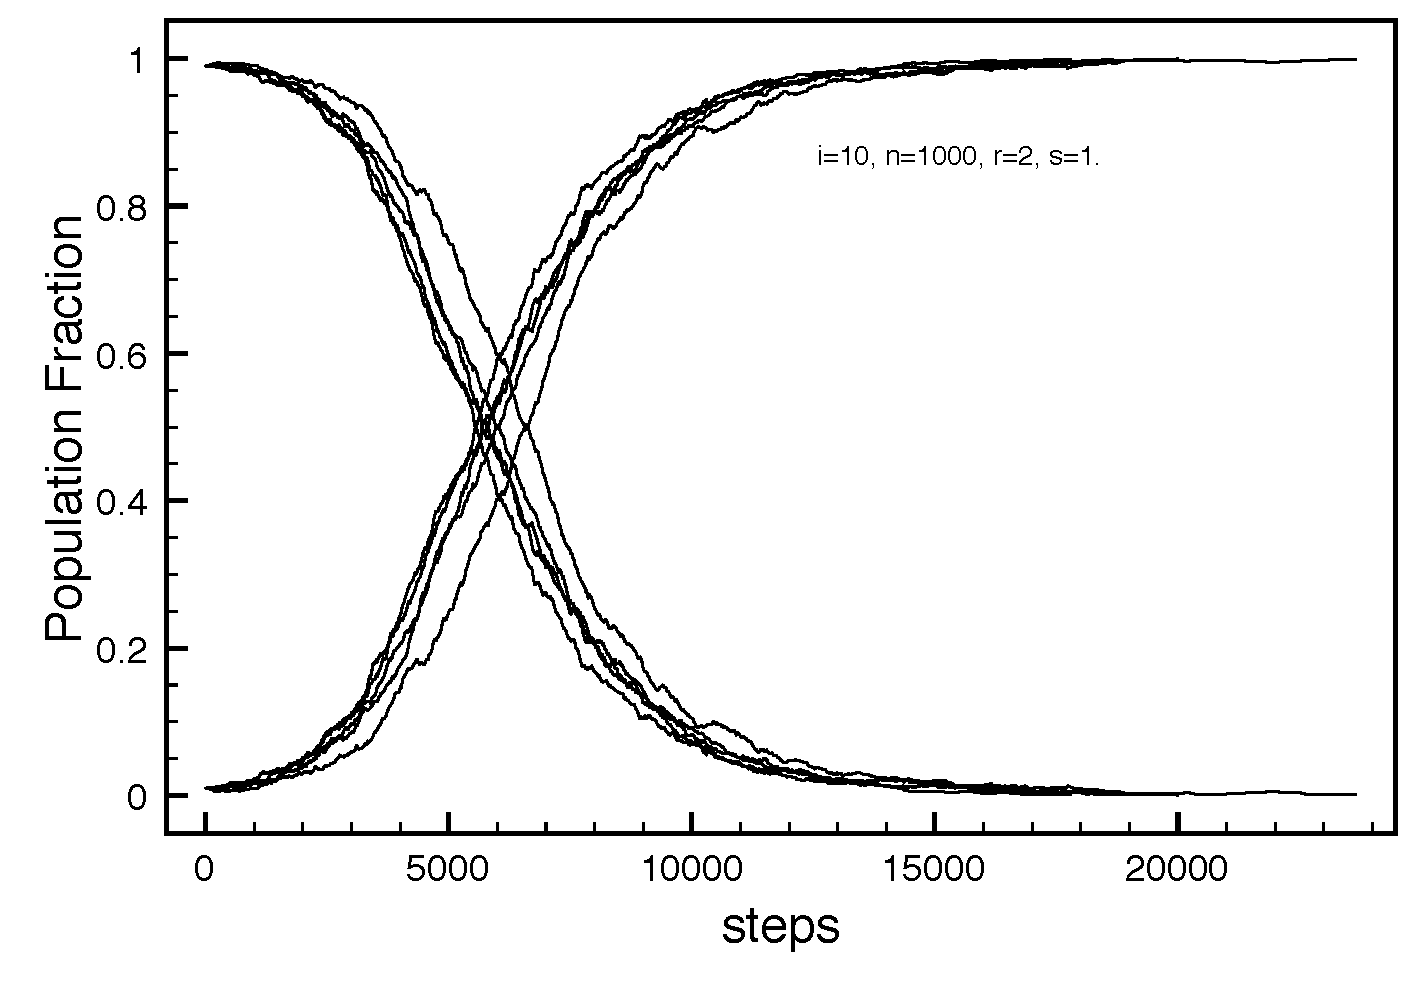
\includegraphics[width=2.5in]{RandomDriftSimulations5.pdf} &
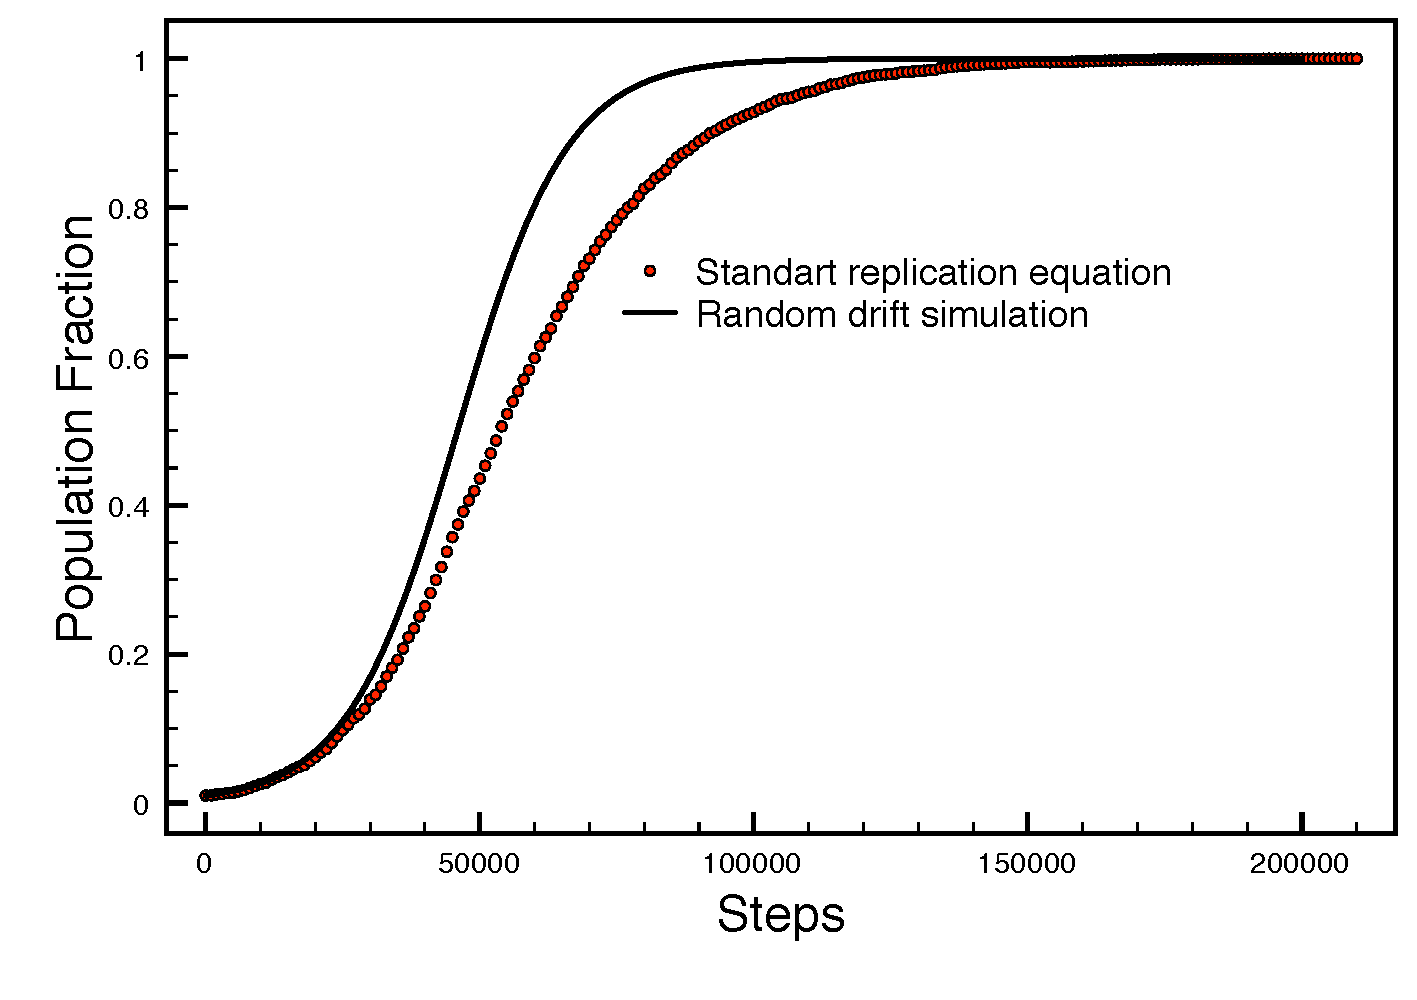
\includegraphics[width=2.5in]{SelectionVsRandom.pdf}
\end{array}$
\end{center}
\caption{Left: Five simulations of random drift for a no so large population $n=1000$. Right: Comparison of random drift and standard replication dynamics(with $t=t' 10000$) for a population of $10000$ and an initial state of $100$ individuals with fitness $r=2$. The other type with $s=1$.}
\label{Fig6.1}
\end{figure}
  
In  Figure \ref{Fig6.2} it is shown how a stochastic simulation for large $n$ population size is close to the deterministic solution of  Eq. \eqref{6.32}, which satisfies the  law of large numbers in stochastic processes.  

  \begin{figure}[H]
  \begin{center}
    \leavevmode
    \ifpdf
      \includegraphics[width=9cm,height=8cm]{DifferentialEquationVsStochastic.pdf}
    \else
      \includegraphics[width=9cm, height=8cm]{DifferentialEquationVsStochastic.pdf}
    \fi
    \caption{In this graph it is shown how the average differential equation fits to a random drift simulation.}
    \label{Fig6.2}
  \end{center}
  \end{figure}

 %%% ----------------------------------------------------------------------

%%% Local Variables: 
%%% mode: latex
%%% TeX-master: "../thesis"
%%% End: 
